\chapter{Логические, продукционные и функциональные модели решения задач в ostis-системах}
\chapauthortoc{Ивашенко В.~П.\\Шункевич Д.~В.\\Василевская А.~П.\\Орлов М.~К.}
\label{chapter_logic_productions}

\begin{SCn}
	\begin{scnrelfromlist}{автор}
		\scnitem{Ивашенко В.~П.}
		\scnitem{Шункевич Д.~В.}
		\scnitem{Василевская А.~П.}
		\scnitem{Орлов М.~К.}
	\end{scnrelfromlist}
\end{SCn}

\bigskip

\abstract{Логические модели решения задач являются основой обработки знаний в интеллектуальных системах. В данной главе рассматривается интеграция различных моделей решения задач, в том числе принципы логического вывода, для решения задач на основе общей формальной модели.}

\bigskip

\begin{SCn}
\begin{scnrelfromlist}{библиографическая ссылка}
	\scnitem{\scncite{Golenkov2001a}}
	\scnitem{\scncite{Golenkov1996_2}}
	\scnitem{\scncite{Orlov2022b}}
	\scnitem{\scncite{Averin2004}}
	\scnitem{\scncite{Golenkov2004}}
	\scnitem{\scncite{Sethy2021}}
	\scnitem{\scncite{Norton2019}}
	\scnitem{\scncite{Yuxuan2022}}
	\scnitem{\scncite{Safawi2015}}
	\scnitem{\scncite{Gungov2018}}
	\scnitem{\scncite{Geramian2017}}
	\scnitem{\scncite{Son2017}}
	\scnitem{\scncite{Lawan2019}}
	\scnitem{\scncite{Uehara2017}}
	\scnitem{\scncite{Lupea2002}}
	\scnitem{\scncite{Weydert2022}}
	\scnitem{\scncite{Chen2021}}
	\scnitem{\scncite{Rybakov2020}}
	\scnitem{\scncite{Gavrilova2001}}
\end{scnrelfromlist}
\end{SCn}

\bigskip

\begin{SCn}
\begin{scnrelfromlist}{подраздел}
	\scnitem{\ref{logic_lang_os}~\nameref{logic_lang_os}}
\end{scnrelfromlist}
\end{SCn}

\section{Операционная семантика логических языков, используемых ostis-системами}
\label{logic_lang_os}

\begin{SCn}
	\begin{scnrelfromlist}{ключевое понятие}
		\scnitem{логический вывод}
		\scnitem{Язык SCL}
		\scnitem{Абстрактная scl-машина}
	\end{scnrelfromlist}
\end{SCn}

\bigskip

\begin{SCn}
	\begin{scnrelfromlist}{ключевое знание}
		\scnitem{Формализация правила вывода Modus ponens}
		\scnitem{Формализация правила резолюции}
		\scnitem{Спецификация агента прямого логического вывода}
	\end{scnrelfromlist}
\end{SCn}

\bigskip

Логика решает задачи доказательства высказываний, аргументации того или иного высказывания, задачу генерации и опровержения гипотез. Некоторые гипотезы могут быть опровергнуты, однако извлекая причины того, почему гипотеза опровергнута, можно изменить посылку гипотезы так, чтобы создать новую гипотезу, которая впоследствии может стать теоремой.

Современная логика изучает формальные языки, служащие для выражения логических рассуждений. Логический язык — формальный язык, предназначенный для воспроизведения логических форм контекстов естественного языка, а также выражения логических законов и способов правильных рассуждений в логических теориях, строящихся в данном языке. Логика не изучает то, как были получены знания, она позволяет представлять знания, а также из существующих знаний вывести новые (то есть из имеющихся формул логики вывести новые формулы этой же логики), установить правильность рассуждений.

На данный момент реализовано много систем логического вывода, использующих известные правила прямого заключения и резолюции в различных видах логик, однако остаются актуальными проблема совместимости вышеописанных систем и проблема коллективного решения задач с использованием различных моделей решения задач.

Каждая модель решения задач задается языком, обеспечивающим представление в памяти кибернетической системы некоторого класса методов решения задач, и интерпретатором указанных методов, определяющим операционную семантику указанного языка. Следует рассмотреть языки, которыми может задаваться логическая модель решения задач. Такими языками являются Rule Interchange Format (RIF), Semantic Web Rule Language (SWRL), SHACL Rules и Notation3 Rules, которые используются в Semantic Web (см. \scncite{Lawan2019}). На рисунке \nameref{fig:swrl_example} представлен пример правил на языке SWRL.

\begin{figure}[http]
	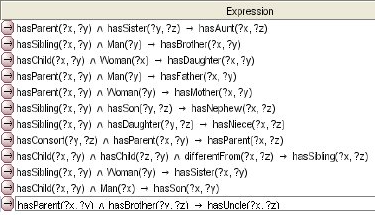
\includegraphics[scale=0.8]{author/part3/figures/swrl_example.png}
	\caption{Запись правил на языке SWRL}
	\label{fig:swrl_example}
\end{figure}

Описанные языки не предусматривают возможность представления формул в различных видах логик, поэтому при помощи них невозможно решить описанные проблемы. Языки правил специально построены для вывода следствий. Синтаксис и семантика языков онтологий и языков правил довольно сильно отличаются, поэтому возникает вопрос, как их совмещать. 

Пролог --- язык и система логического программирования. База знаний системы Пролог содержит информацию в виде предикатов. В логическом программировании, реализованном в Прологе, используется только одно правило вывода --- правило резолюции. Задача пролог-программы заключается в том, чтобы доказать, является ли заданное целевое высказывание следствием из имеющихся формул и, если является, то каким образом был получен такой вывод. Когда пользователь задает вопрос системе Пролог, система ищет соответствующие предикаты в базе знаний и, если они найдены, сравнивать их с заданными условиями. Система Пролог хорошо справляется с нетрудными задачами, однако ограничен лишь одним принципом логического вывода и не позволяет учитывать сложноструктурированные знания в различных видах логик.

Для решения указанных проблем предлагается логический язык на основе SC-кода и абстрактная машина логического вывода на основе предложенного языка. 

Технология OSTIS позволяет интегрировать любые принципы логического вывода для решения задач в интеллектуальных системах на основе общей формальной модели. Для того, чтобы использовать какую-либо новую или существующую модель, необходимо привести ее к предлагаемому формализму, что позволит интегрировать и синхронизировать ее с уже имеющимися в соответствующей библиотеке совместимых компонентов. Формализм SC-кода позволяет описывать широкий спектр понятий и отношений между ними, что делает его подходящим вариантом для реализации логического вывода в интеллектуальных компьютерных системах нового поколения. Кроме того, целесообразно воспользоваться принципом наследования, лежащим в основе иерархической структуризации баз знаний ostis-систем. Исходя из этого предлагается следующая иерархия интегрированных предметных областей:

\begin{SCn}
	\scnheader{Предметная область логических формул, высказываний и формальных теорий}
	\begin{scnrelfromlist}{дочерняя предметная область}
		\scnitem{Предметная область логических языков}
		\scnitem{Предметная область логического вывода}
	\end{scnrelfromlist}
	
	\scnheader{Предметная область логических языков}
	\scnrelfrom{дочерняя предметная область}{Предметная область языка логики высказываний}
	\begin{scnindent}
		\scnrelfrom{дочерняя предметная область}{Предметная область языка логики предикатов}
	\end{scnindent}
	
	\scnheader{Предметная область логических моделей решения задач}
	\begin{scnreltolist}{дочерняя предметная область}
		\scnitem{Предметная область логических языков}
		\scnitem{Предметная область логического вывода}
	\end{scnreltolist}
\end{SCn}

Наследование предметных областей позволяет использовать описанные логики и их компоненты при описании любых логик. Базовые понятия позволяют разработчикам интеллектуальной системы добавлять новые логики. Для реализации конкретной логической модели решения задач необходимо создать предметную область, которая будет дочерней по отношению к \textit{Предметной области логических моделей решения задач} и предметной области некоторого \textit{логического языка}, например, языка логики высказываний, языка логики предикатов, языка нечёткой логики и других.

\textit{Предметная область логических формул, высказываний и формальных теорий} задаёт денотационную семантику логических формул, высказываний и формальных теорий и содержит формальную спецификацию понятий, необходимых для формирования логических формул и высказываний любых логик, в том числе традиционных, нечётких, правдоподбных, темпоральных, логик умолчания и любых других. Логические формулы и высказывания интерпретирубтся с помощью понятий, описанных в \textit{Предметной области логических моделей решения задач}, включающую модель и реализацию абстрактных агентов, необходимых для решения логических задач. Эта предметная область включает в себя спецификацию таких понятий, как логический вывод, правила вывода, равносильные преобразования и аксиомные схемы.

% Источник этого текста и используемых в нём ссылок здесь https://libeldoc.bsuir.by/bitstream/123456789/30629/1/Golenkov_Grapho.pdf
\textbf{Язык SCL} — подъязык SC-кода для записи логических утверждений (см. \scncite{Golenkov1996_2}), он подробно рассматривается в главе \textit{\ref{chapter_logic}~\nameref{chapter_logic}}. Над высказываниями языка SCL можно проводить логический вывод.

Выводом в формальной системе называется любая последовательность формул такая, что любая формула либо аксиома этой формальной системы, либо непосредственное следствие каких-либо предыдущих формул по одному из правил вывода. Идея выводимости центральна в логике: в любой формальной аксиоматической теории теорема --- это формула, которая выводится из аксиом. Правильность умозаключений вводится и проверяется совершенно формально, без какой-либо связи с истинностью входящих в него посылок, то есть исключительно с точки зрения структуры рассуждения. С практической точки зрения самое важное свойство такой формальной правильности рассуждений заключается в следующем: если нам удалось доказать, пользуясь методами формальной логики, правильность рассуждения, и нам известно из опыта, что все используемые посылки истинны, то мы можем быть уверены в истинности заключения (см. \scncite{Averin2004}). Истинность используемых посылок задаётся состоянием базы знаний.

Различные логические подходы позволяют проектировать решатели задач для интеллектуальных систем в разных предметных областях, учитывая их специфику. \textit{Решатель задач} каждой конкретной системы во многом зависит от назначения данной системы, множества решаемых задач, предметной области и других факторов. Некоторые операции, необходимые в одной предметной области будут избыточными в другой. Например, в системе, решающей задачи по геометрии, химии и другим естественным наукам обоснованным будет использование дедуктивных методов вывода, поскольку решение задач в таких предметных областях основывается только на достоверных правилах. В системах же медицинской диагностики, к примеру, постоянно возникает ситуация, когда диагноз может быть поставлен только с некоторой долей уверенности и абсолютно достоверным ответ на поставленный вопрос быть не может. В связи с этим возникает необходимость использования различных решателей задач в различных системах, при этом их состав и возможности в конкретной системе определяется не только непосредственно разработчиком, а требует консультаций с экспертами в данной предметной области. Тем не менее основой для всех видов логик является классическая логика и наиболее общие её методы распространяются на другие логики с некоторыми модификациями, уточнениями и ограничениями (см. \scncite{Golenkov2004}).

Приведем краткую классификацию существующих логических методов решения задач:
\begin{textitemize}
	\item{\textbf{Классический дедуктивный вывод.} Классический дедуктивный вывод является наиболее популярным при построении автоматических решателей задач, так как всегда дает достоверный результат. Дедуктивный вывод включает в себя прямой и обратный и логический вывод (принцип резолюции, процедуру Эрбрана и др.) (см. \scncite{Averin2004}), все виды силлогизмов (см. \scncite{Sethy2021}) и т.д. Основной проблемой дедуктивного вывода является невозможность его использования в ряде случаев, когда отсутствуют достоверные знания.}
	\item{\textbf{Индуктивный вывод.} Индуктивный вывод предоставляет возможность в процессе решения использовать различные предположения, что делает его удобным для использования в слабоформализованных и трудноформализуемых предметных областях, например при построении систем медицинской диагностики. Подробно принципы индуктивного вывода рассмотрены в работах \scncite{Norton2019}, \scncite{Yuxuan2022}.}
	\item{\textbf{Абдуктивный вывод.} Под абдуктивным выводом в искусственном интеллекте, как правило, понимается вывод наилучшего абдуктивного объяснения, т.е. объяснения некоторого события, ставшего неожиданным для системы. Причем наилучшим считается такое объяснение, которое удовлетворяет специальным критериям, определяемым в зависимости от решаемой задачи и используемой	формализации. Абдуктивный вывод подробно рассматривается в работах \scncite{Safawi2015}, \scncite{Gungov2018}.}
	\item{\textbf{Нечеткая логика.} Теория нечетких множеств и, соответственно, нечетких логик, также применяется в системах, связанных с трудноформализуемыми предметными областями (см. \scncite{Geramian2017}, \scncite{Son2017}). Здесь импликативные высказывания могут рассматриваться как "если истинна посылка"{}, то с некоторой вероятностью (часто или редко) истинно заключение, в отличие от классической логики, где зачастую используются статические предметные области и выражение "часто или редко"{} не применимо (корректно использовать только наречие "всегда"{}). Подробнее теория нечетких логик рассматривается в работе \scncite{Uehara2017}.}
	\item{\textbf{Логика умолчаний.} Логика умолчаний применяется, в том числе, для того, чтобы оптимизировать процесс рассуждений,	дополняя процесс достоверного вывода вероятностными  предположениями в тех случаях, когда вероятность ошибки крайне мала. Подробнее логика умолчаний рассмотрена в статьях \scncite{Lupea2002}, \scncite{Weydert2022}.}
	\item{\textbf{Темпоральная логика.} Применение темпоральной логики является очень актуальным для нестатичных предметных областей, в которых истинность того или иного утверждения меняется со временем, что существенно влияет на ход решения какой-либо задачи (см. \scncite{Chen2021}, \scncite{Rybakov2020}). Следует отметить, что используемый в данной работе язык представления знаний предоставляет все необходимые возможности для описания таких динамических предметных областей.}
\end{textitemize}

База знаний интеллектуальной системы включает в себя как модель фактографических знаний о предметной области, для которой предназначена система, так и модель знаний, включающая в себя логические формулы об этой предметной области (аксиомы, теоремы и правила вывода).

\textbf{Абстрактная scl-машина} является машиной логического вывода и относится к классу абстрактных sc-машин (см. \scncite{Golenkov1996_2}). Внутренним языком scl-машины является указанный выше графовый логический язык SCL, её операции соответствуют правилам логического вывода. Семейство специализированных абстрактных графодинамических машин обработки знаний является формальным уточнением операционной семантики указанных выше специализированных графовых языков представления знаний, каждому из которых соответствует одна или несколько абстрактных машин. Эти абстрактные машины соответствуют различным моделям решения задач, различным логикам, различным моделям правдоподобных рассуждений. 
Агент из семейства агентов логического вывода может представлять собой какое-либо правило вывода, которое можно применять для решения логической задачи. Кроме того, необходимы агенты для выполнения равносильных преобразований логической формулы (например, записать формулу эквиваленции как конъюнкцию двух дизъюнкций) и другие агенты, помогающие применять правила вывода на множестве формул языка логики (см. \scncite{Orlov2022b}).

% Показать разные scl-машины в разных логиках. Дедуктивный вывод это база
\begin{SCn}
	\scnheader{Абстрактная scl-машина}
	\begin{scnrelfromset}{декомпозиция абстрактного sc-агента}
		\scnitem{Абстрактный sc-агент применения правила вывода}
		\scnitem{Абстрактный sc-агент эквивалентных преобразований логической формулы}
		\scnitem{Абстрактный sc-агент прямого логического вывода}
		\scnitem{Абстрактный sc-агент обратного логического вывода}	
	\end{scnrelfromset}
\scnhaselement{Реализации интерпретатора логических моделей решения задач}
\begin{scnindent}
	\scnidtf{Реализация scl-машины}
	\scntext{адрес компонента}{https://github.com/ostis-ai/scl-machine}
\end{scnindent}
\end{SCn}

Задачей Абстрактного sc-агента применения правила вывода является применение заданного правила вывода с заданными логическими формулами. Данный sc-агент активируется при появлении в sc-памяти инициированного действия, принадлежащего классу \textit{действие применение правила вывода}. После проверки sc-агентом условия инициирования выполняется процесс применения правила вывода, который заключается в  проверке, существует ли в sc-памяти структуры, соответствующие условию применения данного правила и генерации sc-конструкций в соответствии с применяемым правилом. В ходе работы агента автоматически выполняется процедура унификации: переменные соответствуют константам, константы соответствуют самим себе. Агент применения правила вывода зачастую используется в процессе работы агентов прямого логического вывода, обратного логического вывода и других агентов. Примером правила вывода может быть правило прямого заключения (Modus ponens), представленное на рисунке \nameref{fig:modus_ponens_formalization}.

\begin{figure}[http]
	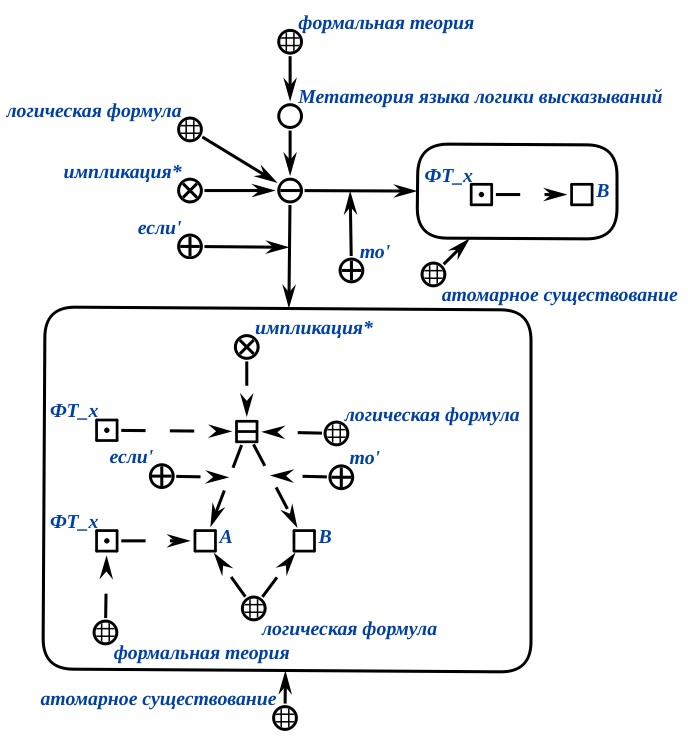
\includegraphics[scale=0.8]{author/part3/figures/Modus_ponens.png}
	\caption{Формализация правила вывода Modus ponens}
	\label{fig:modus_ponens_formalization}
\end{figure}

Можно привести ещё целый ряд высказываний, которые описывают общие свойства всевозможных формальных теорий, каждая из которых описывает ту или иную предметную область. Свойства всевозможных формальных теорий описываются в рамках специальной метатеории для которой совокупность всевозможных формальных теорий является описываемой предметной областью.

Задачей Абстрактного sc-агента эквивалентных преобразований логической формулы является применение некоторых правил, которые приводят логическую формулу в определённый вид. Данный sc-агент активируется при появлении в sc-памяти инициированного действия, принадлежащего классу \textit{действие эквиалентное преобразование логической формулы}. После проверки sc-агентом условия инициирования выполняется процесс преобразования формулы из одной формы в другую, при этом никакие новые знания в sc-памяти с точки зрения исследуемой предметной области не генерируются. Ответом данного агента является множество формул, эквивалентных по смыслу, но различных по форме представления. Такими формами могут быть, например, конъюнктивная нормальная форма или дизъюнктивная нормальная форма. Агент эквивалентных преобразований зачастую вызывается в процессе работы агента применения правила вывода, так как логические формулы не всегда находятся в той форме, которая доступна для применения того или иного правила вывода, однако может быть приведена к нужной форме.

Задачей Абстрактного sc-агента прямого логического вывода является генерации новых знаний на основе некоторых логических утверждений. Данный sc-агент активируется при появлении в sc-памяти инициированного действия, принадлежащего классу \textit{действие прямого логического вывода}. После проверки sc-агентом условия инициирования выполняется процесс прямого логического вывода, который состоит из циклических операций применения правил вывода, генерации новых знаний в sc-памяти и проверки некоторого условия, например, появление в памяти sc-элементов из целевой sc-структуры (см. \scncite{Gavrilova2001}). Входными аргументами такого агента является целевая структура, множество формул, которые используются в ходе вывода агентом применения правил вывода, множество правил вывода, входная структура и выходная структура. В результате выполнения агентом логического вывода действия, в sc-памяти формируется sc-структура, представляющая собой дерево решения. Это дерево состоит из последовательности узлов, представляющих собой применённые правила, которые привели к появлению в sc-памяти требуемых знаний. Такое дерево может быть пустым в случае, если требуемую структуру не удалось сгенерировать в ходе логического вывода. На рисунке \nameref{fig:direct_inference_agent} приведён пример спецификации агента прямого логического вывода.

\begin{figure}[http]
	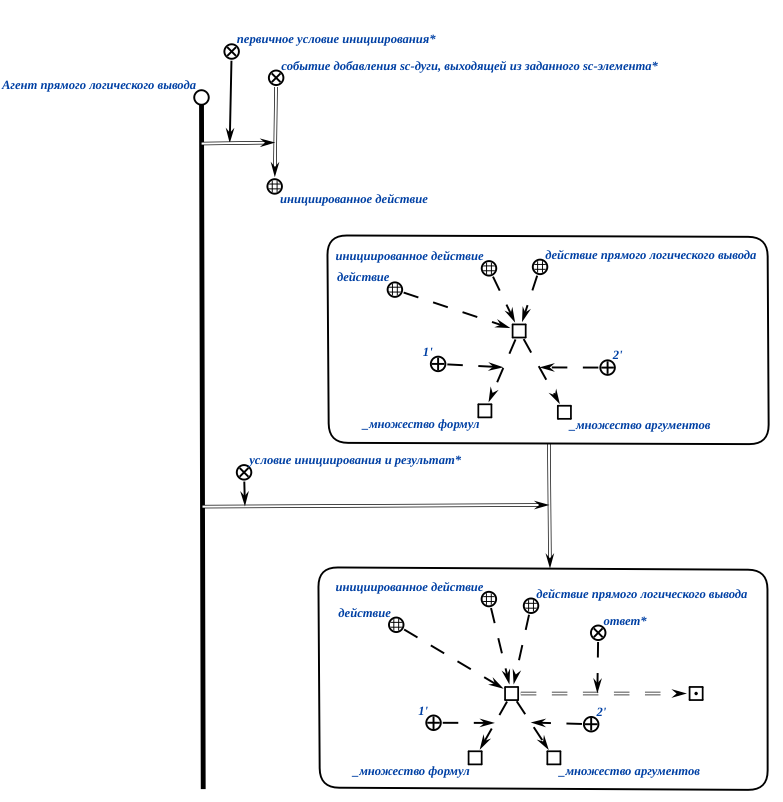
\includegraphics[scale=0.8]{author/part3/figures/direct_inference_agent.png}
	\caption{Спецификация агента прямого логического вывода}
	\label{fig:direct_inference_agent}
\end{figure}

Задачей Абстрактного sc-агента обратного логического вывода является проверка гипотез. Некоторые гипотезы могут быть опровергнуты, однако извлекая причины того, почему гипотеза опровергнута, можно изменить посылку гипотезы так, чтобы создать новую гипотезу, которая впоследствии может стать полезной теоремой. Данный sc-агент активируется при появлении в sc-памяти инициированного действия, принадлежащего классу \textit{действие обратного логического вывода}. После проверки sc-агентом условия инициирования выполняется процесс обратного логического вывода, который схож с процессом прямого логического вывода за исключением того, что поиск правил основывается не на посылках формул, а на их следствиях (см.  \scncite{Gavrilova2001}). Ответом данного агента будет также дерево вывода, которое показывает, с использованием каких правил можно доказать или опровергнуть выдвинутую гипотезу.

\begin{SCn}
	\scnheader{Абстрактный sc-агент эквивалентных преобразований логической формулы}
	\begin{scnrelfromset}{декомпозиция абстрактного sc-агента}
		\scnitem{Абстрактный sc-агент преобразования формулы в конъюнктивную нормальную форму}
		\scnitem{Абстрактный sc-агент преобразования формулы в дизъюнктивную нормальную форму}
		\scnitem{Абстрактный sc-агент применения законов Де Моргана}
		\scnitem{Абстрактный sc-агент эквивалентных преобразований логической формулы по определению}
		\scnitem{Абстрактный sc-агент применения свойств отрицания логических формул}
		\scnitem{Абстрактный sc-агент применения закона идемпотентности логических формул}
		\scnitem{Абстрактный sc-агент применения закона коммутативности логических формул}
		\scnitem{Абстрактный sc-агент применения закона ассоциативности логических формул}
		\scnitem{Абстрактный sc-агент применения закона поглощения логических формул}
		\scnitem{Абстрактный sc-агент применения закона противоречия логических формул}
		\scnitem{Абстрактный sc-агент применения закона двойного отрицания логических формул}
		\scnitem{Абстрактный sc-агент применения закона расщепления логических формул}
	\end{scnrelfromset}
\end{SCn}

Любая формула семантически эквивалентна некоторой формуле в конъюнктивной нормальной форме, в связи с этим иногда удобно применять правило резолюции. Используя законы Де Моргана можно также получить формулы, пригодные для использования правила резолюции.
С помощью правила резолюции можно эффективно доказывать формулы языка логики высказываний.

Однако ничего принципиально нового правильно резолюции не привносит, поскольку формула $A \Rightarrow B$  равносильно $\neg A \lor B$ и из выводимости A и $A \rightarrow B$ следует выводимость B.

\begin{figure}[H]
	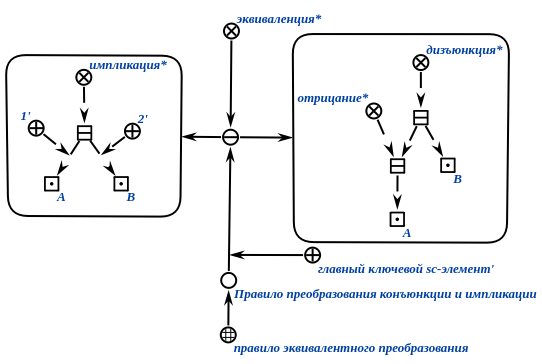
\includegraphics[scale=0.6]{author/part3/figures/conjunction_implication_rule.png}
	\caption{Формализация конъюнктивной нормальной формы для импликации}
	\label{fig:conjunction_implication_rule}
\end{figure}

Если в любых двух дизъюнктах $C_1$ и $C_2$ имеется пара формул $A$ и $\neg A$, то можно сформировать новый дизъюнкт из оставшихся частей изначальных дизъюнктов.

\begin{figure}[H]
	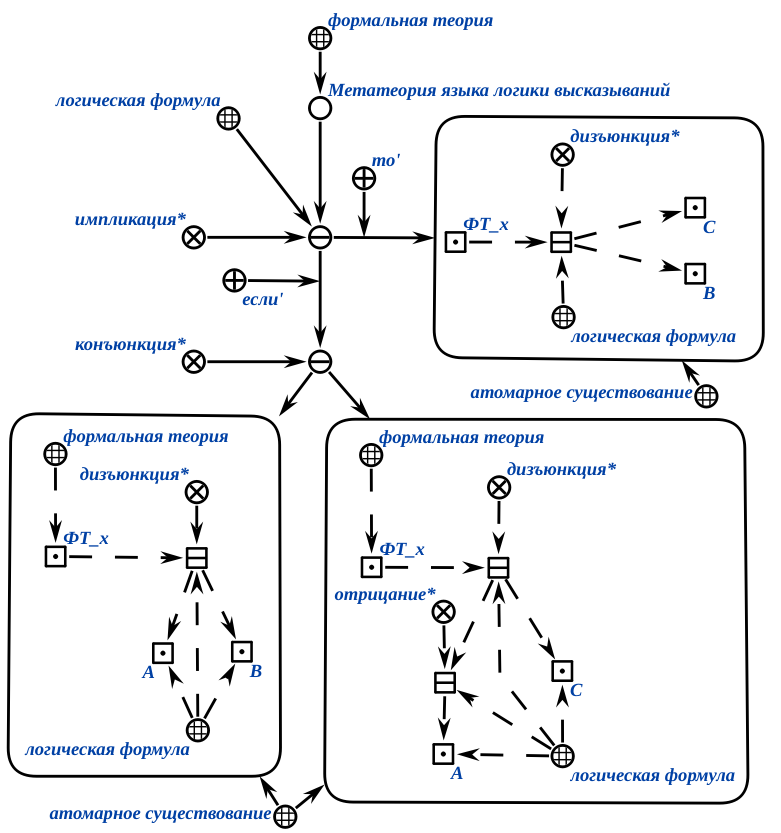
\includegraphics[scale=0.6]{author/part3/figures/resolution.png}
	\caption{Формализация правила резолюции}
	\label{fig:resolution}
\end{figure}

Приведём пример вывода формулы из множества посылок, используя правило резолюции.
Если команда A выигрывает в футбол, то город A' торжествует, а если выигрывает команда B, то торжествовать будет город B'. Выиграть может или только город A', или только город B'. Однако, если выигрывает команда A, то город B' не торжествует, а если выигрывает команда B, то не торжествует город A'. Следовательно, город B' торжествует тогда и только тогда, когда не будет торжествовать город A'. Цель логического вывода - удостовериться, что город B' торжествует тогда и только тогда, когда не будет торжествовать город A'. Доказать вывода формулы равносильно доказательству противоречивости вывода отрицания этой формулы. При использовании правила резолюции это особенно удобно использовать.
Формализация логических формул, соответствующих примеру приведена на рисунке \nameref{fig:resolution_formulas_example}. Каждая неатомарная формула на рисунке принадлежит некоторой формальной теории, то есть считается истинной.

\begin{figure}[H]
	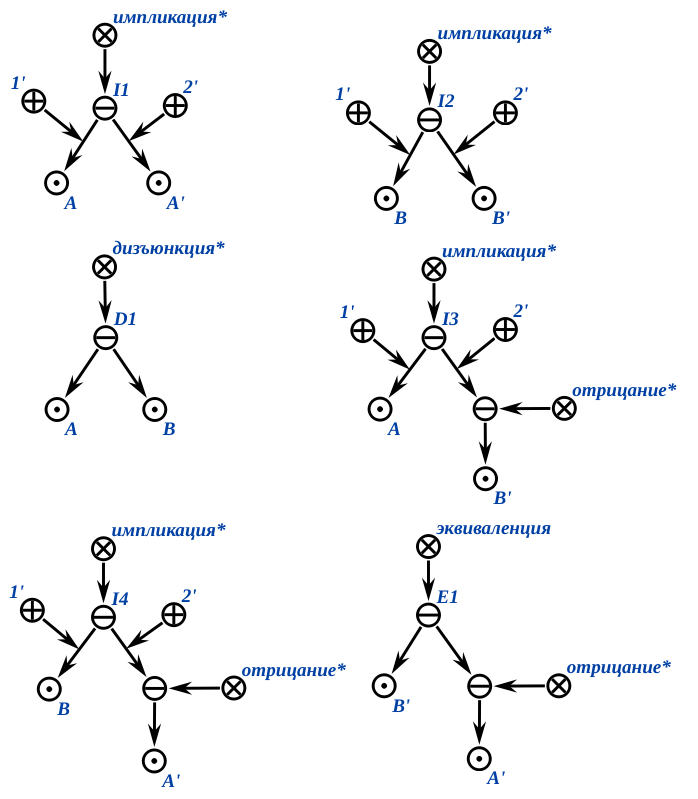
\includegraphics[scale=0.8]{author/part3/figures/resolution_formulas_example.png}
	\caption{Формализация правил для применения правила резолюции}
	\label{fig:resolution_formulas_example}
\end{figure}

Структура A представляет собой атомарную логическую формулу, которая обозначает победу команды A, структура A' представляет формулу, обозначающую торжество города A'. Соответственно, то же самое для структур B и B'.
Выразим логические формулы в булевом базисе. Прежде всего необходимо привести импликацию в конъюнктивную нормальную форму по формуле \nameref{fig:conjunction_implication_rule} и эквиваленцию по определению. Затем применим отрицание к формуле, которую необходимо вывести (эвиваленция). В результате получим следующие формулы (рисунок \nameref{fig:resolution_prepared_formulas}):

\begin{figure}[H]
	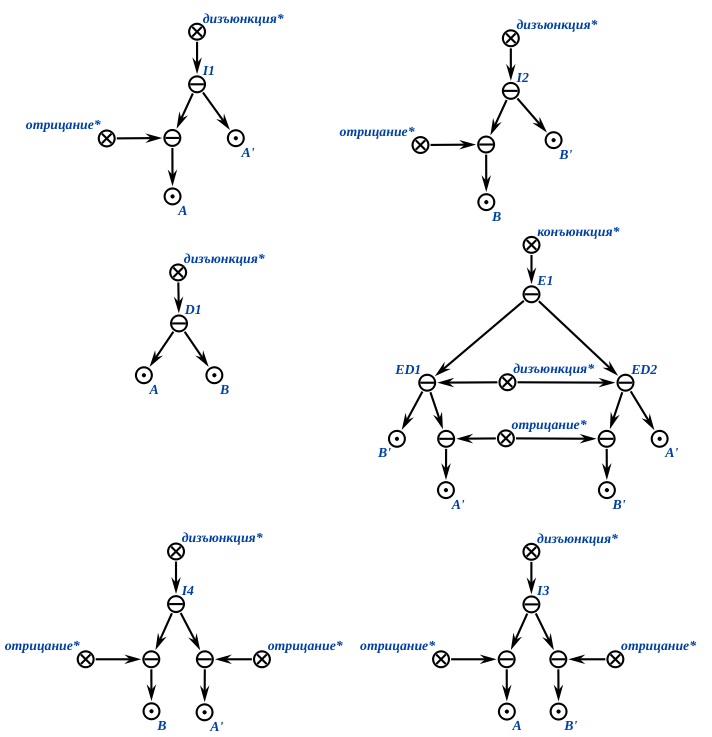
\includegraphics[scale=0.8]{author/part3/figures/resolution_prepared_formulas_example.png}
	\caption{Формализация правил для применения правила резолюции после преобразования в конъюнктивную нормальную форму}
	\label{fig:resolution_prepared_formulas}
\end{figure}

Далее применяя правило резолюции для преобразованных формул получаем пустой дизъюнкт, что говорит о противоречивости множества формул и доказывает формулу эквиваленции о том, что город B' торжествует тогда и только тогда, когда не будет торжествовать город A'.

\begin{figure}[H]
	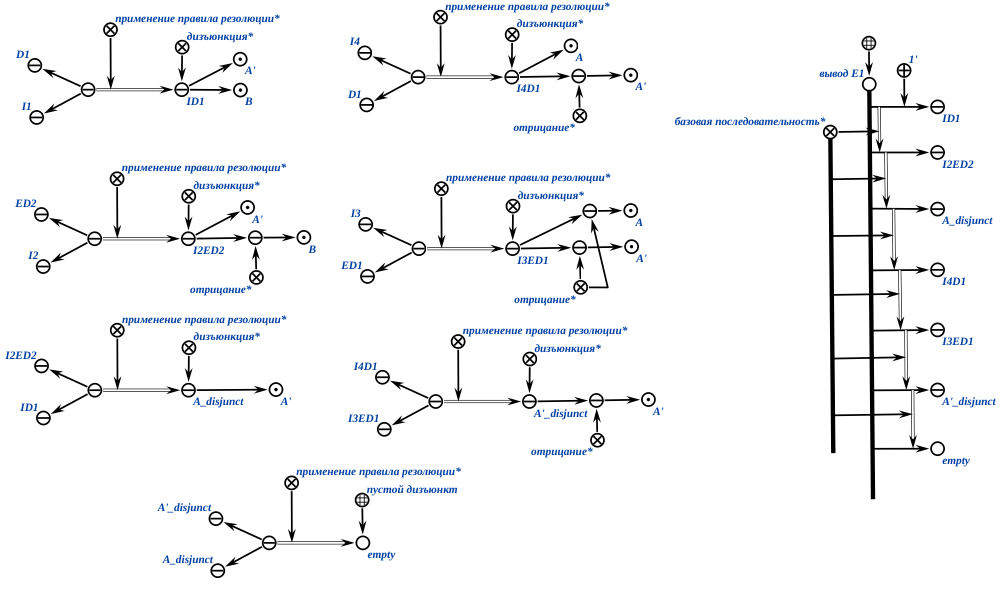
\includegraphics[scale=0.7]{author/part3/figures/resolution_inference.png}
	\caption{Применение принципа резолюции}
	\label{fig:resolution_inference}
\end{figure}

Таким образом, можно использовать различные правила вывода, различные агенты логического вывода в различных видах логик в зависимости от специфики предметной области, в которой решается задача. Каждая модель является совместимой в рамках общей формальной модели решателей задач ostis-систем.

\section{Языки продукционного программирования, используемые ostis-системами}
\subsection{Синтаксис языков продукционного программирования, используемых ostis-системами}
\subsection{Денотационная семантика языков продукционного программирования, используемых ostis-системами}
\subsection{Операционная семантика языков продукционного программирования, используемых ostis-системами}

%%%%%%%%%%%%%%%%%%%%%%%%% referenc.tex %%%%%%%%%%%%%%%%%%%%%%%%%%%%%%
% sample references
% %
% Use this file as a template for your own input.
%
%%%%%%%%%%%%%%%%%%%%%%%% Springer-Verlag %%%%%%%%%%%%%%%%%%%%%%%%%%
%
% BibTeX users please use
% \bibliographystyle{}
% \bibliography{}
%
\biblstarthook{In view of the parallel print and (chapter-wise) online publication of your book at \url{www.springerlink.com} it has been decided that -- as a genreral rule --  references should be sorted chapter-wise and placed at the end of the individual chapters. However, upon agreement with your contact at Springer you may list your references in a single seperate chapter at the end of your book. Deactivate the class option \texttt{sectrefs} and the \texttt{thebibliography} environment will be put out as a chapter of its own.\\\indent
References may be \textit{cited} in the text either by number (preferred) or by author/year.\footnote{Make sure that all references from the list are cited in the text. Those not cited should be moved to a separate \textit{Further Reading} section or chapter.} If the citatiion in the text is numbered, the reference list should be arranged in ascending order. If the citation in the text is author/year, the reference list should be \textit{sorted} alphabetically and if there are several works by the same author, the following order should be used:
\begin{enumerate}
\item all works by the author alone, ordered chronologically by year of publication
\item all works by the author with a coauthor, ordered alphabetically by coauthor
\item all works by the author with several coauthors, ordered chronologically by year of publication.
\end{enumerate}
The \textit{styling} of references\footnote{Always use the standard abbreviation of a journal's name according to the ISSN \textit{List of Title Word Abbreviations}, see \url{http://www.issn.org/en/node/344}} depends on the subject of your book:
\begin{itemize}
\item The \textit{two} recommended styles for references in books on \textit{mathematical, physical, statistical and computer sciences} are depicted in ~\cite{science-contrib, science-online, science-mono, science-journal, science-DOI} and ~\cite{phys-online, phys-mono, phys-journal, phys-DOI, phys-contrib}.
\item Examples of the most commonly used reference style in books on \textit{Psychology, Social Sciences} are~\cite{psysoc-mono, psysoc-online,psysoc-journal, psysoc-contrib, psysoc-DOI}.
\item Examples for references in books on \textit{Humanities, Linguistics, Philosophy} are~\cite{humlinphil-journal, humlinphil-contrib, humlinphil-mono, humlinphil-online, humlinphil-DOI}.
\item Examples of the basic Springer style used in publications on a wide range of subjects such as \textit{Computer Science, Economics, Engineering, Geosciences, Life Sciences, Medicine, Biomedicine} are ~\cite{basic-contrib, basic-online, basic-journal, basic-DOI, basic-mono}. 
\end{itemize}
}

\begin{thebibliography}{99.}%
% and use \bibitem to create references.
%
% Use the following syntax and markup for your references if 
% the subject of your book is from the field 
% "Mathematics, Physics, Statistics, Computer Science"
%
% Contribution 
\bibitem{science-contrib} Broy, M.: Software engineering --- from auxiliary to key technologies. In: Broy, M., Dener, E. (eds.) Software Pioneers, pp. 10-13. Springer, Heidelberg (2002)
%
% Online Document
\bibitem{science-online} Dod, J.: Effective substances. In: The Dictionary of Substances and Their Effects. Royal Society of Chemistry (1999) Available via DIALOG. \\
\url{http://www.rsc.org/dose/title of subordinate document. Cited 15 Jan 1999}
%
% Monograph
\bibitem{science-mono} Geddes, K.O., Czapor, S.R., Labahn, G.: Algorithms for Computer Algebra. Kluwer, Boston (1992) 
%
% Journal article
\bibitem{science-journal} Hamburger, C.: Quasimonotonicity, regularity and duality for nonlinear systems of partial differential equations. Ann. Mat. Pura. Appl. \textbf{169}, 321--354 (1995)
%
% Journal article by DOI
\bibitem{science-DOI} Slifka, M.K., Whitton, J.L.: Clinical implications of dysregulated cytokine production. J. Mol. Med. (2000) doi: 10.1007/s001090000086 
%
\bigskip

% Use the following (APS) syntax and markup for your references if 
% the subject of your book is from the field 
% "Mathematics, Physics, Statistics, Computer Science"
%
% Online Document
\bibitem{phys-online} J. Dod, in \textit{The Dictionary of Substances and Their Effects}, Royal Society of Chemistry. (Available via DIALOG, 1999), 
\url{http://www.rsc.org/dose/title of subordinate document. Cited 15 Jan 1999}
%
% Monograph
\bibitem{phys-mono} H. Ibach, H. L\"uth, \textit{Solid-State Physics}, 2nd edn. (Springer, New York, 1996), pp. 45-56 
%
% Journal article
\bibitem{phys-journal} S. Preuss, A. Demchuk Jr., M. Stuke, Appl. Phys. A \textbf{61}
%
% Journal article by DOI
\bibitem{phys-DOI} M.K. Slifka, J.L. Whitton, J. Mol. Med., doi: 10.1007/s001090000086
%
% Contribution 
\bibitem{phys-contrib} S.E. Smith, in \textit{Neuromuscular Junction}, ed. by E. Zaimis. Handbook of Experimental Pharmacology, vol 42 (Springer, Heidelberg, 1976), p. 593
%
\bigskip
%
% Use the following syntax and markup for your references if 
% the subject of your book is from the field 
% "Psychology, Social Sciences"
%
%
% Monograph
\bibitem{psysoc-mono} Calfee, R.~C., \& Valencia, R.~R. (1991). \textit{APA guide to preparing manuscripts for journal publication.} Washington, DC: American Psychological Association.
%
% Online Document
\bibitem{psysoc-online} Dod, J. (1999). Effective substances. In: The dictionary of substances and their effects. Royal Society of Chemistry. Available via DIALOG. \\
\url{http://www.rsc.org/dose/Effective substances.} Cited 15 Jan 1999.
%
% Journal article
\bibitem{psysoc-journal} Harris, M., Karper, E., Stacks, G., Hoffman, D., DeNiro, R., Cruz, P., et al. (2001). Writing labs and the Hollywood connection. \textit{J Film} Writing, 44(3), 213--245.
%
% Contribution 
\bibitem{psysoc-contrib} O'Neil, J.~M., \& Egan, J. (1992). Men's and women's gender role journeys: Metaphor for healing, transition, and transformation. In B.~R. Wainrig (Ed.), \textit{Gender issues across the life cycle} (pp. 107--123). New York: Springer.
%
% Journal article by DOI
\bibitem{psysoc-DOI}Kreger, M., Brindis, C.D., Manuel, D.M., Sassoubre, L. (2007). Lessons learned in systems change initiatives: benchmarks and indicators. \textit{American Journal of Community Psychology}, doi: 10.1007/s10464-007-9108-14.
%
%
% Use the following syntax and markup for your references if 
% the subject of your book is from the field 
% "Humanities, Linguistics, Philosophy"
%
\bigskip
%
% Journal article
\bibitem{humlinphil-journal} Alber John, Daniel C. O'Connell, and Sabine Kowal. 2002. Personal perspective in TV interviews. \textit{Pragmatics} 12:257--271
%
% Contribution 
\bibitem{humlinphil-contrib} Cameron, Deborah. 1997. Theoretical debates in feminist linguistics: Questions of sex and gender. In \textit{Gender and discourse}, ed. Ruth Wodak, 99--119. London: Sage Publications.
%
% Monograph
\bibitem{humlinphil-mono} Cameron, Deborah. 1985. \textit{Feminism and linguistic theory.} New York: St. Martin's Press.
%
% Online Document
\bibitem{humlinphil-online} Dod, Jake. 1999. Effective substances. In: The dictionary of substances and their effects. Royal Society of Chemistry. Available via DIALOG. \\
http://www.rsc.org/dose/title of subordinate document. Cited 15 Jan 1999
%
% Journal article by DOI
\bibitem{humlinphil-DOI} Suleiman, Camelia, Daniel C. O'Connell, and Sabine Kowal. 2002. `If you and I, if we, in this later day, lose that sacred fire...': Perspective in political interviews. \textit{Journal of Psycholinguistic Research}. doi: 10.1023/A:1015592129296.
%
%
%
\bigskip
%
%
% Use the following syntax and markup for your references if 
% the subject of your book is from the field 
% "Computer Science, Economics, Engineering, Geosciences, Life Sciences"
%
%
% Contribution 
\bibitem{basic-contrib} Brown B, Aaron M (2001) The politics of nature. In: Smith J (ed) The rise of modern genomics, 3rd edn. Wiley, New York 
%
% Online Document
\bibitem{basic-online} Dod J (1999) Effective Substances. In: The dictionary of substances and their effects. Royal Society of Chemistry. Available via DIALOG. \\
\url{http://www.rsc.org/dose/title of subordinate document. Cited 15 Jan 1999}
%
% Journal article by DOI
\bibitem{basic-DOI} Slifka MK, Whitton JL (2000) Clinical implications of dysregulated cytokine production. J Mol Med, doi: 10.1007/s001090000086
%
% Journal article
\bibitem{basic-journal} Smith J, Jones M Jr, Houghton L et al (1999) Future of health insurance. N Engl J Med 965:325--329
%
% Monograph
\bibitem{basic-mono} South J, Blass B (2001) The future of modern genomics. Blackwell, London 
%
\end{thebibliography}
